% !TeX encoding = UTF-8
% !TeX spellcheck = es_ES
% !TeX root = Thermal.tex
%!TEX root=Thermal.tex
El objetivo de este documento es tener un listado de empaquetados de chips usables segun
la potencia que pueden disipar. En este apartado exponemos como calcular la temperatura de un
chip cualquiera.

La forma de modelar/estimar que temperatura alcanzara el silicio en un chip es considerar
la potencia que disipa como una fuente de corriente y el camino que tiene hasta el aire como
una resistencia, segun el modelo simplificado(a)\ref{fig:ThermalEquivalent}.

Antes de ver el modelo simplificado y hacer algunos calculos, veamos un modelo más completo.

\subsection{Modelos mas completos}
Estos modelos los podemos complicar un poco más\sidenote{Acercandose más
a la realidad}, dependiendo de si usamos un dispador sobre un componente o 
usamos la propia PCB como disipador. En cuyo caso la resitencia termica es
de $\SI{100}{\degree\kelvin/\square{inch}}$ o $\SI{645.16}{\degree\kelvin/\square\cm}$.
Aunque estos valores dependeran en gran medida de los materiales usados en la 
fabricacion de la PCB.


\begin{figure}[H]
    \centering
    % !TeX encoding = UTF-8
% !TeX spellcheck = es_ES
% !TeX root = ../Thermal.tex
%!TEX root=../Thermal.tex

\begin{tikzpicture}[american]
    %\draw (0,0) circle[radius=1pt];
    \begin{scope}[shift={(-3,0)}]
        %\draw (0,0) circle[radius=1pt];
        %\draw (-3.25,-5.5) rectangle +(6.5,11);
			
			\draw (-2.75,4.5)
				to[isource, l=$W$ ] ++(2.5,0) 
				node [red, right] {$T_{j}$}
				to [R,l=$R_{thJC}$] ++(0,-2.5) 
					coordinate(TC)
				node[red,left]{$T_{case}$}
				to [R,l=$R_{thCA}$] ++ (0,-4)
					coordinate(TA)
				node[red,left]{$T_{amb}$}
				to[vsource,v=$T_{amb}$] ++(0,-2.5)
				node[ground]{};
			\draw (TC) to[short,*-] ++(2,0)
				to[R,l=$R_{thS}$] ++(0,-2.)
				to[R,l=$R_{thHS}$] ++(0,-2.)
				to[short,-*](TA);
			\node[] at (0,-5.5){a) Componente TH};
     \end{scope}
	  \begin{scope}[shift={(5,0)}]
			%\draw (-5.25,-5.5) rectangle +(10.5,11);
			
			\draw (-4.75,4.5)
				to[isource, l=$W$ ] ++(2.5,0)
					coordinate(TJ) 
				node [red, above] {$T_{j}$}
				to [R,l=$R_{thJC}$] ++(0,-2.5) 
					coordinate(TC)
				node[red,left]{$T_{case}$}
				to [R,l=$R_{thCA}$] ++ (0,-4)
					coordinate(TA)
				node[red,left]{$T_{amb}$}
				to[vsource,v=$T_{amb}$] ++(0,-2.5)
				node[ground]{};
			\draw (TJ) to[short,*-] ++(2.5,0)
				to[R,l=$R_{thJL}$] ++(0,-2.5)
					coordinate(TL)
					node[red,right]{$T_l$}
				to[R,l=$R_{thLC}$] (TC);
			\draw (TL) to [R,l=$R_{thS}$] ++ (0,-2)
					coordinate(Ttop)
					node[red,left]{$T_{top}$}
				to[R,l=$R_{thTopPcb}$]++(0,-2)
				to[short,-*](TA);
			\draw (Ttop) to [vsource,v_=$\SI{10}{\degree\kelvin}$] ++(3,0)
			node[red,right ]{$T_{bott}$}
			to[R,l=$R_{thBottPcb}$] ++(0,-2)
			to[short,-*] (TA)
			;

			%\draw (TC) to[short,*-] ++(2,0)
			%	to[R,l=$R_{thS}$] ++(0,-2.)
			%	to[R,l=$R_{thHS}$] ++(0,-2.)
			%	to[short,-*](TA);
			
			\node[] at (0,-5.5){b) SMD usando PCB como Disipador};
     \end{scope}

\end{tikzpicture}
    \caption{Diseño más complejo}
    \label{fig:ThermalEquivFull}
\end{figure}

Donde $R_{thS}$ es la resistencia termica entre la carcasa y el disipador, $R_{thJL}$ es la
resistencia del silicio a pin (Lead). Asi mismo $R_{thSn}$ es la resistencia entre el pin
y el plano de cobre PCB, que dependera del estaño (Sn) utilizado. Por otra parte $R_{thFr}$
denota la resistencia termica del FR4 en una PCB de dos caras. Por ultimo $R_{thXPcb}$ es la
resistencia termica de las capas de cobre, que depende directamente del tamaño del area.
Nos faltaria una resistencia del pin a la carcasa ($R_{thLC}$), pero podemos considerar que el fabricante ya lo includio en $R_{thJC}$ y que se puede considerar un circuito abierto.

Ahora es momento de implificar el circutito teniendo en cuenta la regla del 10
\sidenote{En realidad depende de la tolerancia}. pudiendo eliminar una resistencia
si hay otra 10 veces mas grande o pequeña segun sea el caso:
\begin{itemize}
    \item \textbf{En serie}: Si $R_p$ es 10 menor que $R_g$, podemos eliminarla puesto que 
    $R_p$ se esconderia en la tolerancia de $R_g$.

    En nuestro caso sucede con $R_{thS}$,$R_{thSn}$, siendo, repsecivamente, estas la pasta
    termica que se pone entre un chip y el dispador, y el estaño que une un pad a la PCB.
    ambas cercanas a \SI{1}{\degree\kelvin/\watt}
    \item \textbf{En paralelo}: Si $R_g$ es los suficientemente grande, su valor se esconderia
    en la tolerancia de $R_p$, por lo que puede eleminarse. Para el calculo de temperaturas, donde nuestro
    origen es una fuente de calor representada como fuente de corriente, lo que hace es "<robar">
    un poco de corriente a $R_p$, por lo que al eleminar $R_g$ tendremos un error al alza. 
    Habiendo calculado una temperatura superior a la real, y si esta es segura, la real tambien.
    
    Asi pues con un disipador correcto ($R_{thHS}$, o la red que representa la PCB), podremos quitar
    $R_{thCA}$.
    \item \textbf{Otras}: Como la conexion en delta, se pueden llegar a simplifcar
    pensando en cuanta corriente se llevan, pero lo normal es que los fabricantes ya
    hayan echo los calculos y no sean necesarios. Como el es el caso de $R_{thLC}$.    
\end{itemize}

\subsection{Origen del modelo}

El modelo aterior\ref{fig:ThermalEquivFull} tiene su orgien en dos tipos de componentes, como ejemplo 
un TO-220 para through hole y un TO-252-3 para SMD. Se han escogido por ser tener una zona
para disipar calor (Tab para TO-220 y un pin/lead en 252). Aunque hay muchos otros empaquetados
que tiene un PAD especifico para disipar calor, normalmente conectado a GND o a otro
plano de potencia.

En la figura siguiente\ref{fig:ThermalModelOrigin} hemos represenado ambos componentes sobre una PCB
de dos caras. Y con flechas verdes los caminos del calor. Asi pues cada flecha es una resistencia "<termica">

\begin{figure}[H]
    \centering
    % !TeX encoding = UTF-8
% !TeX spellcheck = es_ES
% !TeX root = ../Thermal.tex
%!TEX root=../Thermal.tex

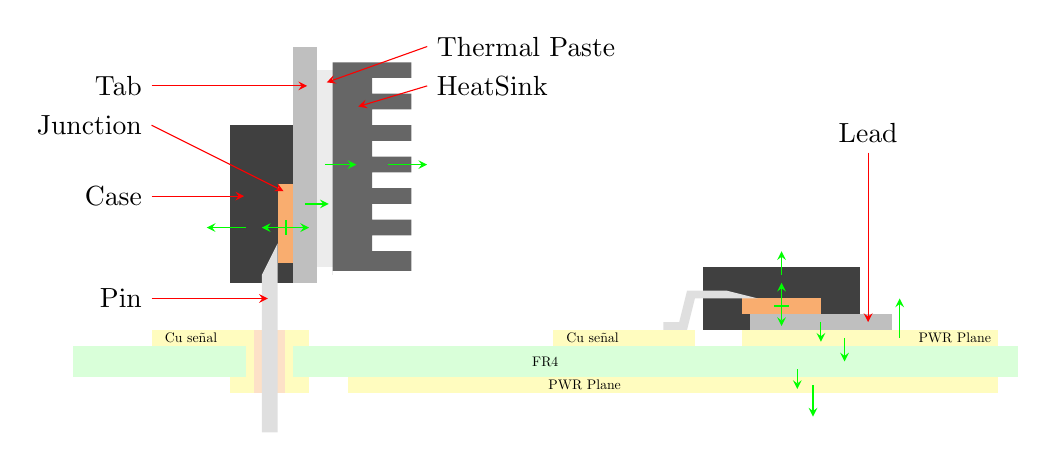
\begin{tikzpicture}[]

	\draw[draw=none,fill=green!15] (-6,-.2) rectangle +(12,.4);
	\draw[draw=none, fill=yellow!25] (-5,0.2) rectangle +(2,.2);
	\draw[draw=none, fill=yellow!25] (-2.5,-0.4) rectangle +(8.25,0.2);

	\node[scale=0.5] at(0,0){FR4};
	\node[scale=0.5] at (-4.5,.3){Cu señal};
	\node[scale=0.5] at (0.5,-.3){PWR Plane};
	\begin{scope}[shift={(-1,0)}]
		% TO-220
		\draw[draw=none,fill=black!75] (-3,1) rectangle +(.8,2);
		\draw[draw=none,fill=gray!50] (-2.2,1) rectangle + (0.3,3);
		\draw[draw=none, fill=Apricot] (-2.4,1.25) rectangle +(.2,1);
		\draw[draw=none,fill=gray!15] (-1.9,1.2) rectangle +(0.2,2.5);
		\draw[draw=none,fill=black!60](-1.7,1.1) -- ++(0,2.7)
		-- ++(1,0) -- ++(0,-.2) -- ++(-0.5,0) -- ++(0,-0.2)
		-- ++(0.5,0) -- ++(0,-.2) -- ++(-0.5,0) -- ++(0,-0.2)
		-- ++(0.5,0) -- ++(0,-.2) -- ++(-0.5,0) -- ++(0,-0.2)
		-- ++(0.5,0) -- ++(0,-.2) -- ++(-0.5,0) -- ++(0,-0.2)
		-- ++(0.5,0) -- ++(0,-.2) -- ++(-0.5,0) -- ++(0,-0.2)
		-- ++(0.5,0) -- ++(0,-.2) -- ++(-0.5,0) -- ++(0,-0.2)
		-- ++(0.5,0) -- ++(0,-.25) -- ++(-1,0);
		\draw[draw=none,fill=yellow!25] (-2.3,-0.4) rectangle +(0.1,0.6);
		\draw[draw=none,fill=yellow!25] (-2.8,-0.4) rectangle +(0.1,0.6);
		\draw[draw=none,fill=yellow!25] (-3,-0.4) rectangle +(1,0.2);
		\draw[draw=none,fill=Apricot!35] (-2.7,-.4) rectangle +(0.4,0.8);
		\draw[draw=none, fill=gray!25] (-2.4,1.5) -- ++(-.2,-.4) -- ++(0,-2) -- ++(0.2,0) -- ++(0,2.4);
		
		\node(th-J) at (-2.2,2.1){};
		\node(th-Tab) at (-1.9,3.5){};
		\node(th-Case) at (-2.7,2.1){};
		\node(th-Pin) at (-2.4,0.8){};

		\node(th-Tp) at (-1.9,3.5){};
		\node(th-HS) at (-1.5,3.2){};
		
		\draw[green,|-stealth] (-2.3,1.7) -- ++(0.3,0);
		\draw[green,-stealth] (-2.05,2) -- ++(0.3,0);
		\draw[green,-stealth] (-1.8,2.5) -- ++(0.4,0);
		\draw[green,-stealth] (-1.,2.5) -- ++(.5,0);

		\draw[green,-stealth] (-2.3,1.7) -- ++(-0.3,0);
		\draw[green,-stealth] (-2.8,1.7) -- ++(-0.5,0);
		

	\end{scope}
	\begin{scope}[shift={(3,.4)}]
		\draw[draw=none,fill=black!75] (-1,0) rectangle +(2,.8);
		\draw[draw=none,fill=gray!50] (-.4,0) rectangle +(1.8,.2);

		\draw[draw=none, fill=Apricot] (-0.5,.2) rectangle +(1,.2);
		\draw[draw=none, fill=gray!25] (-0.3,.4) -- ++(-.4,0.1)
		-- ++(-.5,0) -- ++(-.1,-.4) -- ++(-.2,0) -- ++(0,-.1)
		-- ++(.3,0) -- ++(.1,.4) -- ++(0.8,0);
		\draw [draw=none, fill=yellow!25] (-2.9,0) rectangle +(1.8,-0.2);
		\draw [draw=none, fill=yellow!25] (-0.5,0) rectangle +(3.25,-0.2);
		\node[scale=0.5] at (-2.4,-.1){Cu señal};
		\node[scale=0.5] at (2.2,-.1){PWR Plane};

		\draw[green, |-stealth] (-0,0.3) -- ++(0,0.3);
		\draw[green,-stealth] (0,0.7) -- ++(0,0.3);
		\draw[green, |-stealth] (-0,0.3) -- ++(0,0-.25);
		\draw[green,-stealth] (0.5,0.1) -- ++(0,-0.25);
		\draw[green,-stealth] (0.8,-0.1) -- ++(0,-0.3);
		\draw[green,-stealth] (1.5,-0.1) -- ++(0,0.5);
		\draw[green,-stealth] (0.2,-0.5) -- ++(0,-0.25);
		\draw[green,-stealth] (0.4,-0.7) -- ++(0,-0.4);

		\node(txt-lead) at(1.1,2.5) {Lead};
		\draw[red,-stealth] (txt-lead.south) -- (1.1,0.1);
	\end{scope}

	\node[left](txt-th-J) at (-5,3)  {Junction};
	\node[left](txt-th-Tab) at (-5,3.5)  {Tab};
	\node[left](txt-th-Case) at (-5,2.1)  {Case};
	\node[left](txt-th-Pin) at (-5,0.8)  {Pin};

	\draw[red,-stealth] (txt-th-J.east)-- (th-J);
	\draw[red,-stealth] (txt-th-Tab.east)-- (th-Tab);
	\draw[red,-stealth] (txt-th-Case.east)-- (th-Case);
	\draw[red,-stealth] (txt-th-Pin.east)-- (th-Pin);


	\node[right](txt-th-Tp) at (-1.5,4)  {Thermal Paste};
	\node[right](txt-th-HS) at (-1.5,3.5)  {HeatSink};
	\draw[red,-stealth] (txt-th-Tp.west)-- (th-Tp);
	\draw[red,-stealth] (txt-th-HS.west)-- (th-HS);
\end{tikzpicture}
    \caption{Origen del modelo a partir de componentes}
    \label{fig:ThermalModelOrigin}
\end{figure}

Este modelo se ha basado en la explicacion dada por la AN-2020\cite{TiAN2020} de Texas Instruments.

\subsection{Modelo Simplificado}
El modelo más simplificado es una resistencia, que podremos usarlo cuando este dato nos sea dado
por el fabricante en el DataSheet.
El más realista son dos resistencias en serie, una representado la resistencia desde el silicio al
disipador (ya sea, la carcasa, la pcb o un trozo de metal) y otra de este ultimo al aire.



\begin{figure}[H]
    \centering
    % !TeX encoding = UTF-8
% !TeX spellcheck = es_ES
% !TeX root = ../Thermal.tex
%!TEX root=../Thermal.tex

\begin{tikzpicture}[american]
    %\draw (0,0) circle[radius=1pt];
    \begin{scope}[shift={(-5,0)}]
        %\draw (0,0) circle[radius=1pt];
        %\draw (-2.5,-3.5) rectangle +(5,7);
        
        \draw (-2,2.5) to[isource, l=$W$ ] (0.5,2.5)
            node[right,red]{$T_j$} 
            to[R, l2=$R_{thJA}$ and $\si{\degree\kelvin\per\watt}$] (0.5,-0)
            node[right,red]{$T_{amb}$} 
            to[vsource=$T_a$] (0.5,-2.5)
            node[right,red]{$\SI{0}{\celsius}$} 
            node[ground](gnd){};
        \node at(0,-3.5) {a) Simplificado};
    \end{scope}


    \begin{scope}[shift={(-0,0)}]
        %\draw (0,0) circle[radius=1pt];
        %\draw (-2.5,-4.75) rectangle +(5,9.5);
        
        \draw (-2,3.75) to[isource, l=$W$ ] (0.5,3.75)
            node[right,red]{$T_j$} 
            to[R, l2=$R_{thJC}$ and $\si{\degree\kelvin\per\watt}$] (0.5,1.25)
            node[right,red]{$T_{case}$} 
            to[R, l2=$R_{thCA}$ and $\si{\degree\kelvin\per\watt}$] (0.5,-1.25)
            node[right,red]{$T_{amb}$} 
            to[vsource=$T_a$] (0.5,-3.75)
            node[right,red]{$\SI{0}{\celsius}$} 
            node[ground](gnd){};
        \node at(0,-4.75) {b) Normal};
    \end{scope}

    \begin{scope}[shift={(5,0)}]
        %\draw (0,0) circle[radius=1pt];
        %\draw (-2.5,-3.5) rectangle +(5,7);
        
        \draw (-2,3.75) to[isource, l=$W$ ] (0.5,3.75)
            node[right,red]{$T_j \leq \SI{125}{\celsius}$} 
            to[R, l2=$R_{thHS}$ and $\si{\degree\kelvin\per\watt}$] (0.5,1.25)
            node[right,red]{$T_{case} \leq \SI{100}{\celsius}$} 
            to[R, l2=$R_{thJC}$ and $\si{\degree\kelvin\per\watt}$] (0.5,-1.25)
        
            node[right,red]{$T_{amb}\approx \SI{25}{\celsius}$} 
            to[vsource=$T_a$] (0.5,-3.75)
            node[right,red]{$\SI{0}{\celsius}$} 
            node[ground](gnd){};
        \node at(0,-4.75) {c) Usable};
    \end{scope}

\end{tikzpicture}

    \caption{Circuito Equivalente}
    \label{fig:ThermalEquivalent}
\end{figure}

En la practica es mejor modelar como dos resistencias, una $R_{thJC}$ :
Junction\sidenote{El silicio} a la case\sidenote{Carcasa} y $R_{thCA}$ de la 
carcasa al ambiente, tal y como se representa en el caso (b) \ref{fig:ThermalEquivalent}.
De esta forma podremos variar $R_{thCA}$ con un dispador más grande.

En este modelo es importante mantener la temperatura del silicio $T_j$ por debajo de
$\SI{125}{\celsius}$ lo que se suele corresponde con $T_c=\SI{100}{\celsius}$ en la carcasa.
Como hemos visto, en la realidad, el modelo es más complejo, con resistencias en paralelo segun el dispador
que se ponga, pero se simplifica por la diferencia valores y se puede ignorar $R_{thCA}$
por $R_{thHS}$ del disipador\sidenote{HeatSink}.


\subsection{Calculos en la practica} 
